\documentclass[tikz, border=10pt]{standalone}
\usetikzlibrary{shapes.geometric, arrows.meta, positioning, calc}

\begin{document}

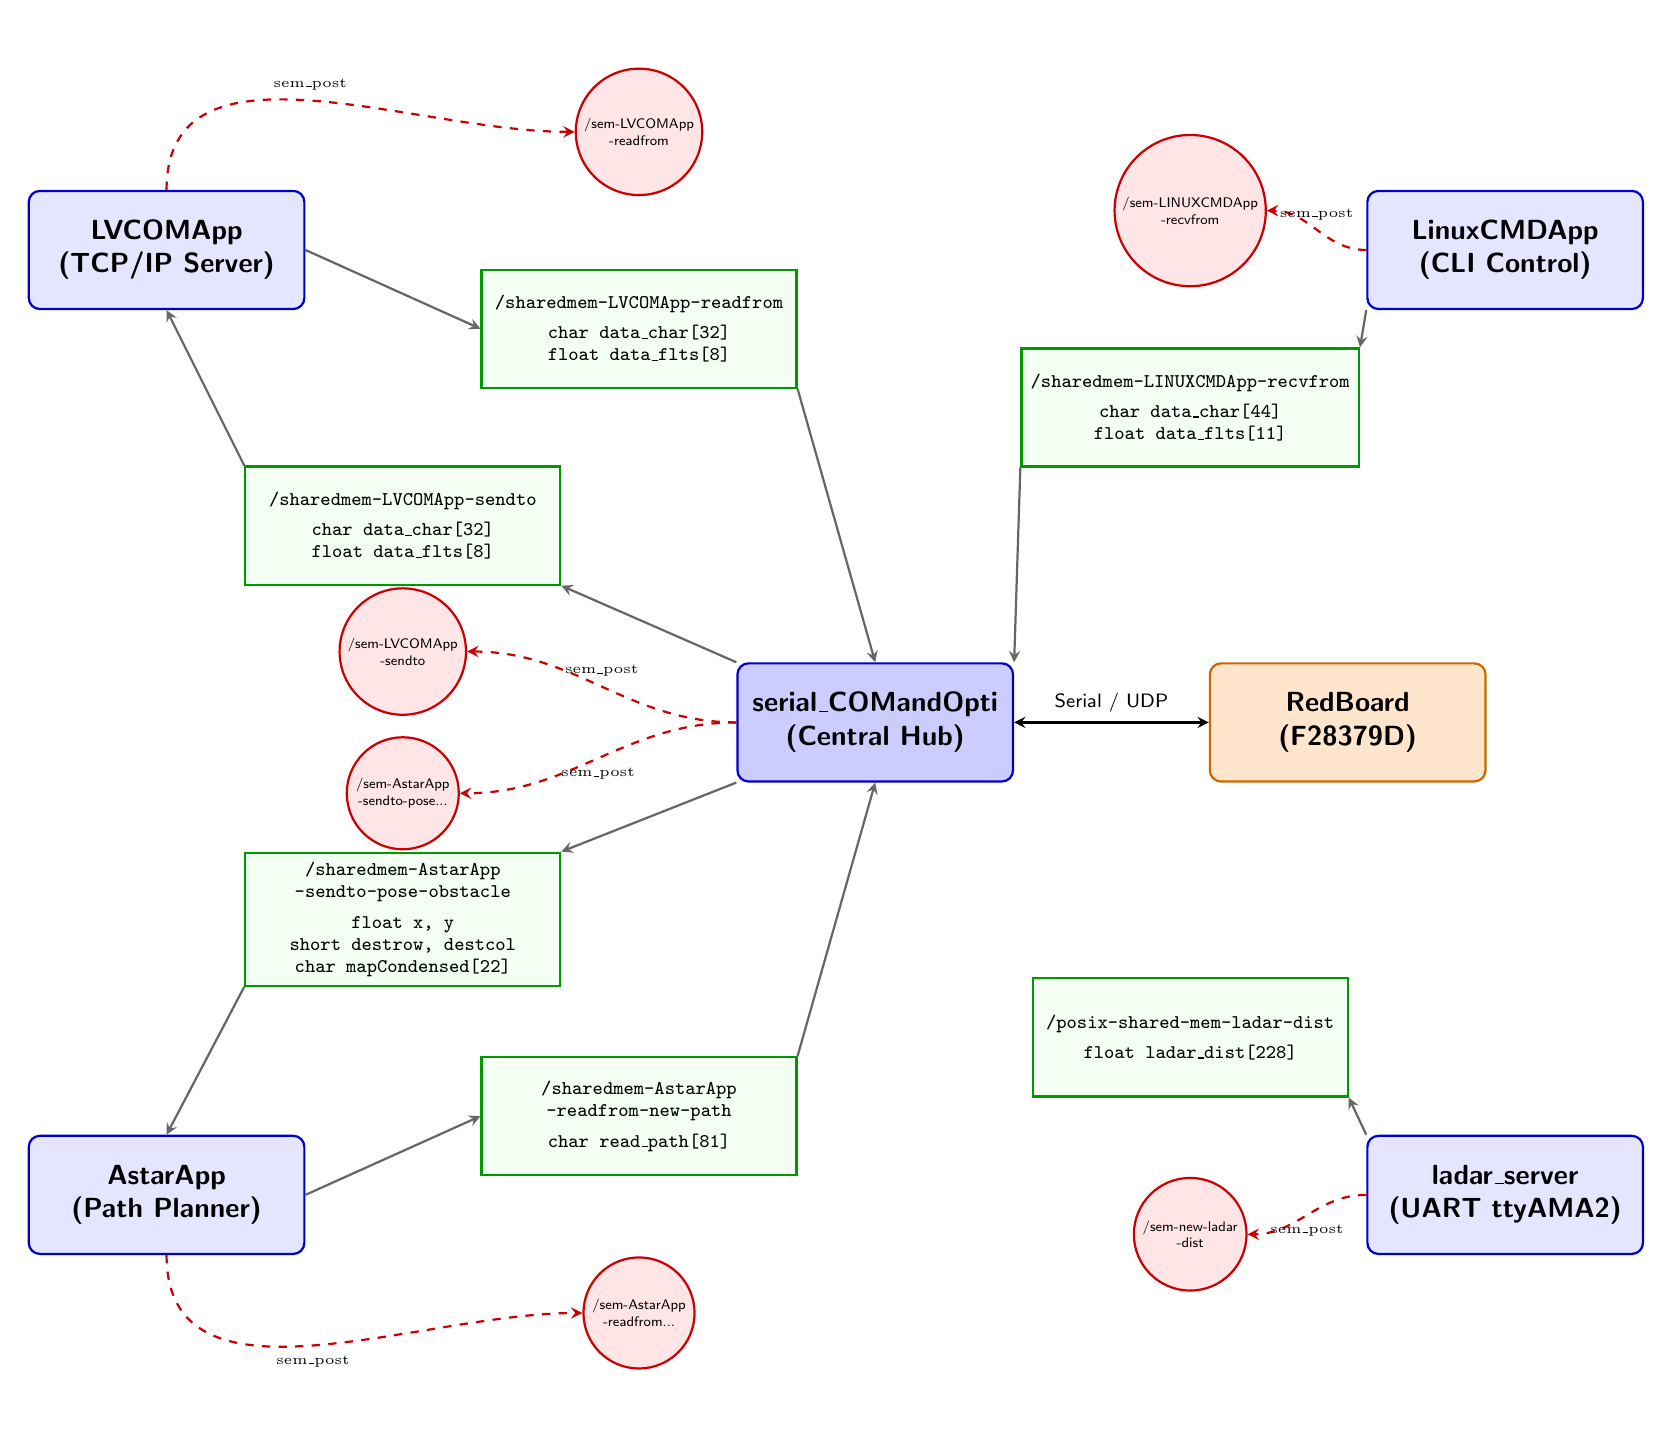
\begin{tikzpicture}[
    >=stealth,
    process/.style={rectangle, rounded corners, draw=blue!80!black, thick, fill=blue!10, minimum width=3.5cm, minimum height=1.5cm, align=center, font=\sffamily\bfseries},
    shm/.style={rectangle, draw=green!60!black, thick, fill=green!5, minimum width=4cm, minimum height=1.5cm, align=center, font=\ttfamily\scriptsize},
    sem/.style={circle, draw=red!80!black, thick, fill=red!10, inner sep=2pt, align=center, font=\sffamily\tiny},
    arrow/.style={->, thick, draw=gray!80!black},
    signal/.style={->, dashed, thick, draw=red!80!black}
]

% Main Hub
\node[process, fill=blue!20] (Hub) at (0, 0) {serial\_COMandOpti\\(Central Hub)};

% ==================== LVCOMApp Block ====================
\node[process] (LVCOM) at (-9, 6) {LVCOMApp\\(TCP/IP Server)};

\node[shm] (shm_lv_recv) at (-3, 5) {/sharedmem-LVCOMApp-readfrom\\[1ex] char data\_char[32] \\ float data\_flts[8]};
\node[sem] (sem_lv_recv) at (-3, 7.5) {/sem-LVCOMApp\\-readfrom};

\node[shm] (shm_lv_send) at (-6, 2.5) {/sharedmem-LVCOMApp-sendto\\[1ex] char data\_char[32] \\ float data\_flts[8]};
\node[sem] (sem_lv_send) at (-6, 0.9) {/sem-LVCOMApp\\-sendto};

% Connections LVCOM <-> Hub
\draw[arrow] (LVCOM.east) -- (shm_lv_recv.west);
\draw[arrow] (shm_lv_recv.south east) -- (Hub.north);
\draw[signal] (LVCOM.north) to[out=90, in=180] node[midway, above, font=\tiny] {sem\_post} (sem_lv_recv.west);

\draw[arrow] (Hub.north west) -- (shm_lv_send.south east);
\draw[arrow] (shm_lv_send.north west) -- (LVCOM.south);
\draw[signal] (Hub.west) to[out=180, in=0] node[midway, above, font=\tiny] {sem\_post} (sem_lv_send.east);


% ==================== LINUXCMDApp Block ====================
\node[process] (CMD) at (8, 6) {LinuxCMDApp\\(CLI Control)};

\node[shm] (shm_cmd_recv) at (4, 4) {/sharedmem-LINUXCMDApp-recvfrom\\[1ex] char data\_char[44] \\ float data\_flts[11]};
\node[sem] (sem_cmd_recv) at (4, 6.5) {/sem-LINUXCMDApp\\-recvfrom};

% Connections CMD <-> Hub
\draw[arrow] (CMD.south west) -- (shm_cmd_recv.north east);
\draw[arrow] (shm_cmd_recv.south west) -- (Hub.north east);
\draw[signal] (CMD.west) to[out=180, in=0] node[midway, above, font=\tiny] {sem\_post} (sem_cmd_recv.east);


% ==================== AstarApp Block ====================
\node[process] (Astar) at (-9, -6) {AstarApp\\(Path Planner)};

\node[shm] (shm_astar_recv) at (-3, -5) {/sharedmem-AstarApp\\-readfrom-new-path\\[1ex] char read\_path[81]};
\node[sem] (sem_astar_recv) at (-3, -7.5) {/sem-AstarApp\\-readfrom...};

\node[shm] (shm_astar_send) at (-6, -2.5) {/sharedmem-AstarApp\\-sendto-pose-obstacle\\[1ex] float x, y \\ short destrow, destcol \\ char mapCondensed[22]};
\node[sem] (sem_astar_send) at (-6, -0.9) {/sem-AstarApp\\-sendto-pose...};

% Connections Astar <-> Hub
\draw[arrow] (Astar.east) -- (shm_astar_recv.west);
\draw[arrow] (shm_astar_recv.north east) -- (Hub.south);
\draw[signal] (Astar.south) to[out=-90, in=180] node[midway, below, font=\tiny] {sem\_post} (sem_astar_recv.west);

\draw[arrow] (Hub.south west) -- (shm_astar_send.north east);
\draw[arrow] (shm_astar_send.south west) -- (Astar.north);
\draw[signal] (Hub.west) to[out=180, in=0] node[midway, below, font=\tiny] {sem\_post} (sem_astar_send.east);


% ==================== LADAR Server Block ====================
\node[process] (Ladar) at (8, -6) {ladar\_server\\(UART ttyAMA2)};

\node[shm] (shm_ladar) at (4, -4) {/posix-shared-mem-ladar-dist\\[1ex] float ladar\_dist[228]};
\node[sem] (sem_ladar) at (4, -6.5) {/sem-new-ladar\\-dist};

% Connections Ladar <-> SHM
\draw[arrow] (Ladar.north west) -- (shm_ladar.south east);
\draw[signal] (Ladar.west) to[out=180, in=0] node[midway, below, font=\tiny] {sem\_post} (sem_ladar.east);

% ==================== RedBoard / F28379D Block ====================
\node[process, fill=orange!20, draw=orange!80!black] (RedBoard) at (6, 0) {RedBoard\\(F28379D)};

% Connection Hub <-> RedBoard
\draw[<->, thick, draw=black] (Hub.east) -- (RedBoard.west) node[midway, above, font=\sffamily\scriptsize, align=center] {Serial / UDP};

\end{tikzpicture}

\end{document}